% !TeX document-id = {be34c84b-deee-4ae7-a020-3510ae5ecf87}
%%% File encoding: UTF-8
%%% äöüÄÖÜß  <-- keine deutschen Umlaute hier? UTF-faehigen Editor verwenden!

%%% Magic Comments zum Setzen der korrekten Parameter in kompatiblen IDEs
% !TeX encoding = utf8
% !TeX program = pdflatex 
% !TeX spellcheck = de_DE
% !BIB program = biber

\documentclass[bachelor,german]{hgbthesis}
% Zulässige Optionen in [..]: 
%   Typ der Arbeit: diploma, master (default), bachelor, internship 
%   Hauptsprache: german (default), english
%%%----------------------------------------------------------

\RequirePackage[utf8]{inputenc}		% bei der Verw. von lualatex oder xelatex entfernen!

\graphicspath{{images/}}    % Verzeichnis mit Bildern und Grafiken
\logofile{}				% Logo-Datei = images/logo.pdf (\logofile{}, wenn kein Logo gewünscht)
\bibliography{references}  	% Biblatex-Literaturdatei (references.bib)

%%%----------------------------------------------------------
\begin{document}
%%%----------------------------------------------------------

\begin{center}
	\begin{Huge}
	Entwickeln von Erweiterungen für Microsoft Dynamics NAV unter Verwendung von ExtensionsV2
	\end{Huge}

	\begin{Large}
	(Exposé) 
	\bigbreak
	Johannes Naderer
	
	(se0307)
	\end{Large}	

	

	
\end{center}
\begin{center}
	
\end{center}
%%%----------------------------------------------------------
\frontmatter                    % Titelei (röm. Seitenzahlen)
%%%----------------------------------------------------------

%\maketitle
%\tableofcontents

%%%----------------------------------------------------------
\mainmatter          % Hauptteil (ab hier arab. Seitenzahlen)
%%%----------------------------------------------------------

\chapter{Thema}
\label{cha:Thema}

In dieser Arbeit soll der Leser schrittweise an das Thema der Erweiterungsentwicklung im ERP-System Microsoft Dynamics NAV eingeführt werden. 
Das Thema der Erweiterungsentwicklung im Dynamics NAV Umfeld wurde erstmals mit Erscheinen der Version 2018 relevant. Für dieses neue Konzept wird seitens Microsoft die neue Sprache \emph{AL} entwickelt, die zwar auf der bisherigen Sprache \emph{C/AL} aufbaut, jedoch einige Einschränkungen und Erweiterungen mit sich bringt. Ziel der neuen Sprache und des Entwicklungsparadigmas rund um sie ist es, Entwicklern einen zeitgemäßen Entwicklungsprozess zu erleichtern und gleichzeitig bereits innerhalb der Sprache Vorkehrungen für den Sprung in die Cloud zu treffen. 
\chapter{Einleitung}
\label{cha:Motivation}

\section{Motivation}
\label{sec:Motivation}
ERP-Systeme sind heute aus dem wirtschaftlichen Umfeld nicht mehr wegzudenken. \cite{WongTein2003} \cite{DuplagaMarzie2003} Wo in den 1970er und 1980er Jahren innerhalb der einzelnen Abteilungen von Unternehmen verschiedene Software-Lösungen verwendet wurden, ist man sich mittlerweile einig, dass eine zentrale Applikation zur Verwaltung aller unternehmerisch wichtigen Daten und Prozessschritte große Vorteile liefert.
Gleichzeitig hatte dieses Umdenken zur Folge, dass kleine Softwarehersteller ins wanken gerieten - da seitens der Wirtschaft allumfassende Software-Giganten gefordert wurden, die mit eingeschränkten Ressourcen und Branchenwissen nicht entwickelt werden konnten. Genau diese Großsysteme werden neben dem Platzhirsch SAP und einigen anderen Unternehmen auch von Microsoft mit seiner Dynamics Sparte geliefert.

Vor der Kaufentscheidung für ein ERP-System gilt es neben den finanziellen Aspekten auch herauszufinden, welche Systeme die bestehenden Prozesse des Unternehmens am Besten abbilden. \cite{WongTein2003} Und genau hier spielt die Anpassbarkeit und Erweiterbarkeit eines Systems eine zentrale Rolle. Systeme bilden oft Geschäftsprozesse auf ihre eigene Art ab, und zwingen so den Anwender bestehende Prozesse anzupassen, oder das System zu ändern. Gerade bei branchenspezifischen Abläufen muss hier meist die Logik des ERP-Systems geändert oder erweitert werden. Solche Änderungen sind jedoch meist teuer und zeitintensiv. Gerade der finanzielle Aufwand einer ERP-Einführung stellt für Unternehmen ein großes Risiko dar. Da der Großteil der großen Systeme darüber hinaus auch periodisch mit Updates versorgt werden, um gegenüber rechtlichen Änderungen flexibel zu bleiben, können sich Eingriffe in die Logik auch negativ auf die Updatefähigkeit des Systems auswirken. 

Um die Aspekte der Erweiterbarkeit und Anpassungsmöglichkeit zu bedienen, entschied sich Microsoft in seinem ERP-System Dynamics NAV bereits in sehr frühen Versionen, zertifizierten Entwicklern freien Zugang zum Applikationscode zu gewähren. \cite{BrummelPatterns2015} So können diese die gesamte Geschäftlogik je nach Anforderung abändern, aushebeln und erweitern. Das hat zum Einen zur Folge, dass Entwickler mächtige Applikationen erstellen können, und sich diese direkt in das bestehende System integrieren lassen, allerdings kommen mit diesen Möglichkeiten auch Probleme auf. Je weiter die oft über Jahrzehnte verwendeten Systeme vom Standardlieferumfang von Microsoft abweichen, desto aufwändiger, teurer und fehleranfälliger ist es diese Systeme mit monatlichen und jährlichen Updates zu versorgen. 

Um dieses Problem anzugehen, und gleichzeitig zukünftige Entwicklungen kompatibel zur Cloud-Variante des ERP-Systems zu halten, wurde mit der Version 2017 erstmals das Konzept der Erweiterungen mit ExtensionsV1 eingeführt. ExtensionsV1 war ein neuer Ansatz für das ERP-System zu programmieren und hatte viele Vorteile, war jedoch in einigen technischen Details noch nicht ausgereift und konnte sich daher gegenüber der konventionellen prozeduralen Entwicklung im Dynamics NAV Umfeld nicht durchsetzen. Mit der in 2018 veröffentlichten Version -- ExtensionsV2 -- wurden nicht nur viele diese Mängel behoben, sondern auch eine neue Sprache mitsamt Entwicklungsumgebung vorgestellt.

\section{Zielsetzung}
\label{sec:Zielsetzung}
Ziel dieser Arbeit ist es, dem Leser einen generellen technischen Überblick über die Architektur des Systems Microsoft Dynamics NAV zu geben. Dafür ist es notwendig, das Prinzip der verwendeten 3-Schichten-Architektur zu verstehen. Zusätzlich wird geklärt, wie und wo C/AL bzw. AL Code kompiliert und schlussendlich ausgeführt wird. 
Anschließend soll die erweiterungsbasierte Programmierung zum bisherigen Ansatz der traditionellen prozeduralen Programmierung verglichen werden. Dazu wird zuerst ein Einblick in die Programmierung in der C/SIDE Entwicklungsumgebung mit der Sprache C/AL an einem einfach gehaltenem Beispiel vermittelt. Danach wird dasselbe Beispiel mit der neuen Sprache AL in Visual Studio Code erstellt. In der anschließenden Diskussion wird dann im Detail auf die Gemeinsamkeiten und Differenzen beiden Arten eingegangen. Hierbei ist es nicht Ziel, syntaktische Kleinigkeiten hervorzuheben, sondern konzeptionelle Unterschiede, und deren Vor-/Nachteile zu beleuchten. 

Der Leser soll nach Durchsicht der Arbeit einen Überblick über das Programmsystem Microsoft Dynamics NAV haben, und die beiden angewandten Programmierkonzepte verstehen und unterscheiden können.



\chapter{Stand der Technik}
\label{cha:standdertechnik}
Microsoft Dynamics NAV hat während seiner Entwicklung einige Architektursprünge hingelegt. Ausgehend von Navision für DOS zum Sprung als reine 2-Schichten-Architektur mit FAT-Client zur heutigen 3-Schichten Architektur. \cite{Sah2016}
\begin{figure}[h]
	\centering\small
	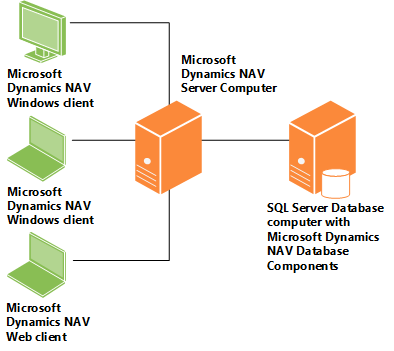
\includegraphics{images/nav_roletailoredarchitecture.png}
	\caption{Overview: Dynamics NAV 3-Tier-Architecture https://docs.microsoft.com/en-us/dynamics-nav/product-and-architecture-overview}
	\label{fig:Image3TierArchitecture}
\end{figure}

Abbildung \ref{fig:Image3TierArchitecture} zeigt einen vereinfachten Grundaufbau der 3-Schichten-Architektur von Dynamics NAV. In Grün sehen wir die verschiedenen Client-Arten die die erste Schicht repräsentieren. Neben dem klassischen Windows-Client zählen auch der Web-Client und die verschiedenen Mobile-Apps zur Schicht Eins. Auf der Schicht Zwei befindet sich der NAV-Server. Dieser bildet den Kern ges Gesamtsystems, verbindet die Datenbank mit den Clients und führt sämtliche Geschäftslogik aus. Die dritte Schicht bildet die Datenbank, auf der sämtliche Datenbestände des Systems verwaltet und persistiert werden. Als Datenbanksystem wird hier Microsoft SQL Server verwendet. 
 Die Serverkomponenten (Server, Datenbank) können sowohl lokal installiert werden, als auch in die Cloud (Microsoft Azure) ausgelagert werden, wobei sämtliche Kombinationen möglich sind, und man daher freie Hand bei der Auswahl der Betriebsoptionen hat.





%%%----------------------------------------------------------
\MakeBibliography                        % Quellenverzeichnis
%%%----------------------------------------------------------

%%% Messbox zur Druckkontrolle ------------------------------


%%%----------------------------------------------------------
\end{document}
%%%----------------------------------------------------------